\documentclass{beamer}\usepackage[]{graphicx}\usepackage[]{color}
% maxwidth is the original width if it is less than linewidth
% otherwise use linewidth (to make sure the graphics do not exceed the margin)
\makeatletter
\def\maxwidth{ %
  \ifdim\Gin@nat@width>\linewidth
    \linewidth
  \else
    \Gin@nat@width
  \fi
}
\makeatother

\definecolor{fgcolor}{rgb}{1, 0.894, 0.769}
\newcommand{\hlnum}[1]{\textcolor[rgb]{0.824,0.412,0.118}{#1}}%
\newcommand{\hlstr}[1]{\textcolor[rgb]{1,0.894,0.71}{#1}}%
\newcommand{\hlcom}[1]{\textcolor[rgb]{0.824,0.706,0.549}{#1}}%
\newcommand{\hlopt}[1]{\textcolor[rgb]{1,0.894,0.769}{#1}}%
\newcommand{\hlstd}[1]{\textcolor[rgb]{1,0.894,0.769}{#1}}%
\newcommand{\hlkwa}[1]{\textcolor[rgb]{0.941,0.902,0.549}{#1}}%
\newcommand{\hlkwb}[1]{\textcolor[rgb]{0.804,0.776,0.451}{#1}}%
\newcommand{\hlkwc}[1]{\textcolor[rgb]{0.78,0.941,0.545}{#1}}%
\newcommand{\hlkwd}[1]{\textcolor[rgb]{1,0.78,0.769}{#1}}%
\let\hlipl\hlkwb

\usepackage{framed}
\makeatletter
\newenvironment{kframe}{%
 \def\at@end@of@kframe{}%
 \ifinner\ifhmode%
  \def\at@end@of@kframe{\end{minipage}}%
  \begin{minipage}{\columnwidth}%
 \fi\fi%
 \def\FrameCommand##1{\hskip\@totalleftmargin \hskip-\fboxsep
 \colorbox{shadecolor}{##1}\hskip-\fboxsep
     % There is no \\@totalrightmargin, so:
     \hskip-\linewidth \hskip-\@totalleftmargin \hskip\columnwidth}%
 \MakeFramed {\advance\hsize-\width
   \@totalleftmargin\z@ \linewidth\hsize
   \@setminipage}}%
 {\par\unskip\endMakeFramed%
 \at@end@of@kframe}
\makeatother

\definecolor{shadecolor}{rgb}{.97, .97, .97}
\definecolor{messagecolor}{rgb}{0, 0, 0}
\definecolor{warningcolor}{rgb}{1, 0, 1}
\definecolor{errorcolor}{rgb}{1, 0, 0}
\newenvironment{knitrout}{}{} % an empty environment to be redefined in TeX

\usepackage{alltt}
\usepackage{../371g-slides}
\usepackage{preview}
\title{Indicator Variables and Interactions}
\subtitle{Lecture 18}
\author{STA 371G}

% This is adapted from http://community.amstat.org/stats101/resources/viewdocument?DocumentKey=e4f8d3f1-41a3-4f01-9f8b-f8fbe1562c15&tab=librarydocuments&CommunityKey=5ad27b39-58d0-49e9-9f6f-0c39c82a0401.
\IfFileExists{upquote.sty}{\usepackage{upquote}}{}
\begin{document}
  
  

\frame{\maketitle}

  % Show outline at beginning of each section
  \AtBeginSection[]{
    \begin{frame}<beamer>
      \tableofcontents[currentsection]
    \end{frame}
  }

  %%%%%%% Slides start here %%%%%%%

  \begin{darkframes}
    \section{Using categorical variables with 2 categories in a regression model}

    \begin{frame}{Housing price data}
      Today we'll consider a 2007 housing price data set from Saratoga County, NY.
      \begin{itemize}
        \item \textbf{Price}: price of house (\$)
        \item \textbf{Living.Area}: amount of living space (sq ft)
        \item \textbf{Fireplace}: whether house has a fireplace (yes/no)
      \end{itemize}

    \end{frame}

    \begin{frame}[fragile]{How much is a fireplace worth?}
\begin{knitrout}
\definecolor{shadecolor}{rgb}{0.137, 0.137, 0.137}\color{fgcolor}\begin{kframe}
\begin{alltt}
\hlkwd{boxplot}\hlstd{(Price} \hlopt{~} \hlstd{Fireplace,} \hlkwc{data}\hlstd{=houses,}
  \hlkwc{col}\hlstd{=}\hlstr{'gray'}\hlstd{,} \hlkwc{ylab}\hlstd{=}\hlstr{'Price'}\hlstd{)}
\end{alltt}
\end{kframe}
\includegraphics[width=\maxwidth]{/tmp/figures/unnamed-chunk-2-1} 

\end{knitrout}
    \end{frame}

    \begin{frame}{Using a categorical variable as a predictor}
      \begin{itemize}[<+->]
        \item We can't just throw a categorical variable into a regression---all $X$'s have to be quantitative
        \item Idea: Recode a binary (yes/no) categorical variable as 0/1
        \item This is called a \alert{indicator variable} or \alert{dummy variable}
        \item Let's set 1 = Yes and 0 = No (doesn't matter; just need to be consistent)
      \end{itemize}
    \end{frame}

    \begin{frame}[fragile]{How much is a fireplace worth?}
      

      If we regress Price on Fireplace, we get the regression equation
      \[
        \widehat{\text{Price}} = 174653 + 65261\cdot(\text{Fireplace = Yes})
      \]
      The average difference between houses with and without a fireplace is \$65261.

      \note{What is the reference level?}
    \end{frame}

    \begin{frame}[fragile]{How much is a fireplace worth?}
      Note that the coefficient represents the difference between the means, and the intercept in the mean price when Fireplace is ``No'':
\begin{knitrout}
\definecolor{shadecolor}{rgb}{0.137, 0.137, 0.137}\color{fgcolor}\begin{kframe}
\begin{alltt}
\hlkwd{tapply}\hlstd{(houses}\hlopt{$}\hlstd{Price, houses}\hlopt{$}\hlstd{Fireplace, mean)}
\end{alltt}
\begin{verbatim}
    No    Yes 
174653 239914 
\end{verbatim}
\begin{alltt}
\hlnum{239914} \hlopt{-} \hlnum{174653}
\end{alltt}
\begin{verbatim}
[1] 65261
\end{verbatim}
\end{kframe}
\end{knitrout}
    \end{frame}

    \section{Using categorical variables with 3+ categories in a regression model}

    \begin{frame}{Using a categorical variable with 3+ categories as a predictor}
      \begin{itemize}
        \item Let's say we want to predict price from type of heat (electric, hot air, hot water)
        \item We CANNOT set 0 = electric, 1 = hot air, 2 = hot water and throw that into the model!
      \end{itemize}
      \pause
\begin{knitrout}
\definecolor{shadecolor}{rgb}{0.137, 0.137, 0.137}\color{fgcolor}
\includegraphics[width=\maxwidth]{/tmp/figures/unnamed-chunk-5-1} 

\end{knitrout}
    \end{frame}

    \begin{frame}{Using a categorical variable with 3+ categories as a predictor}
      \begin{enumerate}
        \item Pick an (arbitrary) \alert{reference category}, say Electric
        \item For the other categories, create an indicator variable that is 1 if the value is that category, and 0 otherwise
        \begin{tabular}{l|ll}
          Value & Heat Type is Hot Air & Heat Type is Hot Water \\ 
          \hline
          Electric & 0 & 0 \\
          Hot Air & 1 & 0 \\
          Hot Water & 0 & 1 \\
        \end{tabular}  
      \end{enumerate}
    \end{frame}

    \begin{frame}[fragile]
      \fontsm
      If you add a categorical variable to a model, R will pick a reference category and create indicator variables for you:
      \fontsize{8}{8}\selectfont
\begin{knitrout}
\definecolor{shadecolor}{rgb}{0.137, 0.137, 0.137}\color{fgcolor}\begin{kframe}
\begin{alltt}
\hlstd{model} \hlkwb{<-} \hlkwd{lm}\hlstd{(Price} \hlopt{~} \hlstd{Heat.Type,} \hlkwc{data}\hlstd{=houses)}
\hlkwd{summary}\hlstd{(model)}
\end{alltt}
\begin{verbatim}

Call:
lm(formula = Price ~ Heat.Type, data = houses)

Residuals:
    Min      1Q  Median      3Q     Max 
-221355  -63355  -17644   43895  548645 

Coefficients:
                   Estimate Std. Error t value     Pr(>|t|)    
(Intercept)          161889       5469   29.60      < 2e-16 ***
Heat.TypeHot Air      64467       6168   10.45      < 2e-16 ***
Heat.TypeHot Water    47244       7754    6.09 0.0000000014 ***
---
Signif. codes:  0 '***' 0 '**' 0 '*' 0 '.' 0 ' ' 1

Residual standard error: 95500 on 1725 degrees of freedom
Multiple R-squared:  0.0597,	Adjusted R-squared:  0.0586 
F-statistic: 54.8 on 2 and 1725 DF,  p-value: <2e-16
\end{verbatim}
\end{kframe}
\end{knitrout}
    \end{frame}

    \begin{frame}{Interpreting indicator variable slopes}
      \begin{itemize}
        \item The slope of an indicator variable represents the predicted difference in $Y$ between the corresponding category and the reference category
        \item Example: The "\texttt{Heat.TypeHot Air}" slope of 64467 represents the predicted difference in prices between houses with hot air heat and houses with electric heat
      \end{itemize}
    \end{frame}

    \begin{frame}
      Regression equation:
      \begin{align*}
      \widehat{\text{Price}} = 161889
      + 64467 \cdot\text{(Heat Type = Hot Air)}  \\
      + 47244 \cdot\text{(Heat Type = Hot Water)}
      \end{align*}

      \vspace{0.3in}\pause
      Let's write out the equations:
      \begin{itemize}[<+->]
        \item Electric $\longrightarrow$
          $ \widehat{\text{Price}} = 161889
          + 64467 \cdot 0
          + 47244 \cdot 0 = 161889$

        \item Hot Air $\longrightarrow$
        $ \widehat{\text{Price}} = 161889
        + 64467 \cdot 1
        + 47244 \cdot 0 = 226355$

        \item Hot Water $\longrightarrow$
        $ \widehat{\text{Price}} = 161889
        + 64467 \cdot 0
        + 47244 \cdot 1 = 209132$
        \end{itemize}
    \end{frame}

    \section{Interactions between a categorical and a quantitative variable}

    \begin{frame}{What is the relationship between price and size?}
\begin{knitrout}
\definecolor{shadecolor}{rgb}{0.137, 0.137, 0.137}\color{fgcolor}
\includegraphics[width=\maxwidth]{/tmp/figures/unnamed-chunk-7-1} 

\end{knitrout}
    \end{frame}

    \begin{frame}{Predicting price from living area}
      \begin{center}
        Let's start by creating a simple regression predicting \\
        price from living area (in sq ft).
      \end{center}
    \end{frame}

    \begin{frame}[fragile]
      \fontsize{8}{8}\selectfont
\begin{knitrout}
\definecolor{shadecolor}{rgb}{0.137, 0.137, 0.137}\color{fgcolor}\begin{kframe}
\begin{alltt}
\hlstd{model1} \hlkwb{<-} \hlkwd{lm}\hlstd{(Price} \hlopt{~} \hlstd{Living.Area,} \hlkwc{data}\hlstd{=houses)}
\hlkwd{summary}\hlstd{(model1)}
\end{alltt}
\begin{verbatim}

Call:
lm(formula = Price ~ Living.Area, data = houses)

Residuals:
    Min      1Q  Median      3Q     Max 
-277022  -39371   -7726   28350  553325 

Coefficients:
            Estimate Std. Error t value Pr(>|t|)    
(Intercept) 13439.39    4992.35    2.69   0.0072 ** 
Living.Area   113.12       2.68   42.17   <2e-16 ***
---
Signif. codes:  0 '***' 0 '**' 0 '*' 0 '.' 0 ' ' 1

Residual standard error: 69100 on 1726 degrees of freedom
Multiple R-squared:  0.507,	Adjusted R-squared:  0.507 
F-statistic: 1.78e+03 on 1 and 1726 DF,  p-value: <2e-16
\end{verbatim}
\end{kframe}
\end{knitrout}
    \end{frame}

    \begin{frame}
      \begin{center}
        Can we do better by adding a dummy variable for fireplace to the model?
      \end{center}
    \end{frame}

    \begin{frame}[fragile]
      \fontsize{8}{8}\selectfont
\begin{knitrout}
\definecolor{shadecolor}{rgb}{0.137, 0.137, 0.137}\color{fgcolor}\begin{kframe}
\begin{alltt}
\hlstd{model2} \hlkwb{<-} \hlkwd{lm}\hlstd{(Price} \hlopt{~} \hlstd{Living.Area} \hlopt{+} \hlstd{Fireplace,} \hlkwc{data}\hlstd{=houses)}
\hlkwd{summary}\hlstd{(model2)}
\end{alltt}
\begin{verbatim}

Call:
lm(formula = Price ~ Living.Area + Fireplace, data = houses)

Residuals:
    Min      1Q  Median      3Q     Max 
-271421  -39935   -7887   28215  554651 

Coefficients:
             Estimate Std. Error t value Pr(>|t|)    
(Intercept)  13599.16    4991.70    2.72   0.0065 ** 
Living.Area    111.22       2.97   37.48   <2e-16 ***
FireplaceYes  5567.38    3716.95    1.50   0.1344    
---
Signif. codes:  0 '***' 0 '**' 0 '*' 0 '.' 0 ' ' 1

Residual standard error: 69100 on 1725 degrees of freedom
Multiple R-squared:  0.508,	Adjusted R-squared:  0.508 
F-statistic:  891 on 2 and 1725 DF,  p-value: <2e-16
\end{verbatim}
\end{kframe}
\end{knitrout}
    \end{frame}

    \begin{frame}
      By adding the dummy variable, we are essentially fitting two regression lines:
\begin{knitrout}
\definecolor{shadecolor}{rgb}{0.137, 0.137, 0.137}\color{fgcolor}
\includegraphics[width=\maxwidth]{/tmp/figures/unnamed-chunk-10-1} 

\end{knitrout}
    They have the same slope, but different intercepts
    \end{frame}

    \begin{frame}{Interactions}
      \begin{center}
        Our regression equation is
        \[
          \widehat{\text{Price}} = 13599
            + 111 \cdot\text{Living.Area}
            + 5567 \cdot\text{FireplaceYes}.
        \]

        \bigskip\pause

        What if the \emph{slope} of the best-fit line is different for houses with a fireplace than for houses without?

        \bigskip\pause

        Equivalently, what if the \emph{effect} of having a bigger house is different for houses with fireplaces than for houses without fireplaces?
      \end{center}
    \end{frame}

    \begin{frame}{Interactions}
      To model this, we can add an \alert{interaction term} that consists of the product of the two predictors:
      \begin{multline*}
        \text{Price} = \beta_0 + \beta_1\cdot\text{Living.Area} + \beta_2\cdot\text{FireplaceYes}
        \\ + \beta_3\cdot\text{Living.Area}\cdot\text{FireplaceYes} + \epsilon_i.
      \end{multline*}

      \pause\bigskip

      Now, the \emph{slope} of Living.Area depends on the \emph{value} of Fireplace!

      \bigskip
      Houses with a fireplace have a slope of of $\beta_1+\beta_3$, houses without have a slope of $\beta_1$.
    \end{frame}

    \begin{frame}[fragile]
      \fontsize{8}{8}\selectfont
\begin{knitrout}
\definecolor{shadecolor}{rgb}{0.137, 0.137, 0.137}\color{fgcolor}\begin{kframe}
\begin{alltt}
\hlstd{model3} \hlkwb{<-} \hlkwd{lm}\hlstd{(Price} \hlopt{~} \hlstd{Living.Area} \hlopt{*} \hlstd{Fireplace,} \hlkwc{data}\hlstd{=houses)}
\hlkwd{summary}\hlstd{(model3)}
\end{alltt}
\begin{verbatim}

Call:
lm(formula = Price ~ Living.Area * Fireplace, data = houses)

Residuals:
    Min      1Q  Median      3Q     Max 
-241710  -39588   -7821   28480  542055 

Coefficients:
                          Estimate Std. Error t value   Pr(>|t|)    
(Intercept)               40901.29    8234.66    4.97 0.00000075 ***
Living.Area                  92.36       5.41   17.07    < 2e-16 ***
FireplaceYes             -37610.41   11024.85   -3.41    0.00066 ***
Living.Area:FireplaceYes     26.85       6.46    4.16 0.00003376 ***
---
Signif. codes:  0 '***' 0 '**' 0 '*' 0 '.' 0 ' ' 1

Residual standard error: 68800 on 1724 degrees of freedom
Multiple R-squared:  0.513,	Adjusted R-squared:  0.512 
F-statistic:  605 on 3 and 1724 DF,  p-value: <2e-16
\end{verbatim}
\end{kframe}
\end{knitrout}
    \end{frame}

    \begin{frame}
      This corresponds to the regression equation:
      \begin{multline*}
        \widehat{\text{Price}} = 40901
          + 92 \cdot\text{Living.Area}
          - 37610 \cdot\text{FireplaceYes} \\
          + 27 \cdot\text{Living.Area}\cdot\text{FireplaceYes}
      \end{multline*}
      \pause
      In other words, for houses without a fireplace:
      \[
        \widehat{\text{Price}} = 40901
        + 92 \cdot\text{Living.Area}
      \]
      \pause
      And for houses with a fireplace:
      \[
        \widehat{\text{Price}} = (40901 - 37610)
        + (92 + 27) \cdot\text{Living.Area}
      \]
    \end{frame}

    \begin{frame}[fragile]{Making predictions}
      Let's make predictions for the price of a 2500 sq ft house, both with and without a fireplace:
\begin{knitrout}
\definecolor{shadecolor}{rgb}{0.137, 0.137, 0.137}\color{fgcolor}\begin{kframe}
\begin{alltt}
\hlkwd{predict}\hlstd{(model3,} \hlkwd{list}\hlstd{(}\hlkwc{Living.Area}\hlstd{=}\hlnum{2500}\hlstd{,} \hlkwc{Fireplace}\hlstd{=}\hlstr{"Yes"}\hlstd{),}
  \hlkwc{interval}\hlstd{=}\hlstr{"prediction"}\hlstd{)}
\end{alltt}
\begin{verbatim}
     fit    lwr    upr
1 301331 166362 436300
\end{verbatim}
\begin{alltt}
\hlkwd{predict}\hlstd{(model3,} \hlkwd{list}\hlstd{(}\hlkwc{Living.Area}\hlstd{=}\hlnum{2500}\hlstd{,} \hlkwc{Fireplace}\hlstd{=}\hlstr{"No"}\hlstd{),}
  \hlkwc{interval}\hlstd{=}\hlstr{"prediction"}\hlstd{)}
\end{alltt}
\begin{verbatim}
     fit    lwr    upr
1 271811 136405 407217
\end{verbatim}
\end{kframe}
\end{knitrout}
      \note{Discuss the meaning of the overlap here}
    \end{frame}

    \begin{frame}
\begin{knitrout}
\definecolor{shadecolor}{rgb}{0.137, 0.137, 0.137}\color{fgcolor}
\includegraphics[width=\maxwidth]{/tmp/figures/unnamed-chunk-13-1} 

\end{knitrout}
    \end{frame}

    \begin{frame}[fragile]{Main effects and interaction effects}
      \fontsize{10}{10}\selectfont
      In the output, the coefficients for Living.Space and Fireplace are \alert{main effects}, and the coefficient for $\text{Living.Space}\cdot\text{Fireplace}$ is an \alert{interaction effect}.

      
\begin{knitrout}
\definecolor{shadecolor}{rgb}{0.137, 0.137, 0.137}\color{fgcolor}\begin{kframe}
\begin{alltt}
\hlkwd{summary}\hlstd{(model3)}\hlopt{$}\hlstd{coefficients}
\end{alltt}
\begin{verbatim}
                         Estimate Std. Error t value Pr(>|t|)
(Intercept)                 40901     8234.7     5.0  7.5e-07
Living.Area                    92        5.4    17.1  1.8e-60
FireplaceYes               -37610    11024.9    -3.4  6.6e-04
Living.Area:FireplaceYes       27        6.5     4.2  3.4e-05
\end{verbatim}
\end{kframe}
\end{knitrout}

      \pause
      The main effect for Living.Area (92.36) represents the predicted incremental effect of each additional square foot of living space, when there is no fireplace present.

      \bigskip\pause
      When we have an interaction term in the model, we \emph{must} include the main effect as well!
    \end{frame}

    \section{Interactions between two quantitative variables}

    \begin{frame}{NBA data}
      Basketball-Reference.com provides detailed data on NBA teams and players. We'll look at team data for 4 seasons ending in 2016; each of these metrics is the average across the season:
      \begin{itemize}
        \item \textbf{PTS}: Total points
        \item \textbf{PCT3P}: Percentage of 3-point shots made
        \item \textbf{N3PA}: Number of 3-point shots attempted
      \end{itemize}
      There are 30 NBA teams $\times$ 4 seasons = 120 cases in this file.
    \end{frame}

    \begin{frame}{NBA data}
      In basketball, there are three ways to score:
      \begin{columns}[onlytextwidth]
        \column{.6\textwidth}
          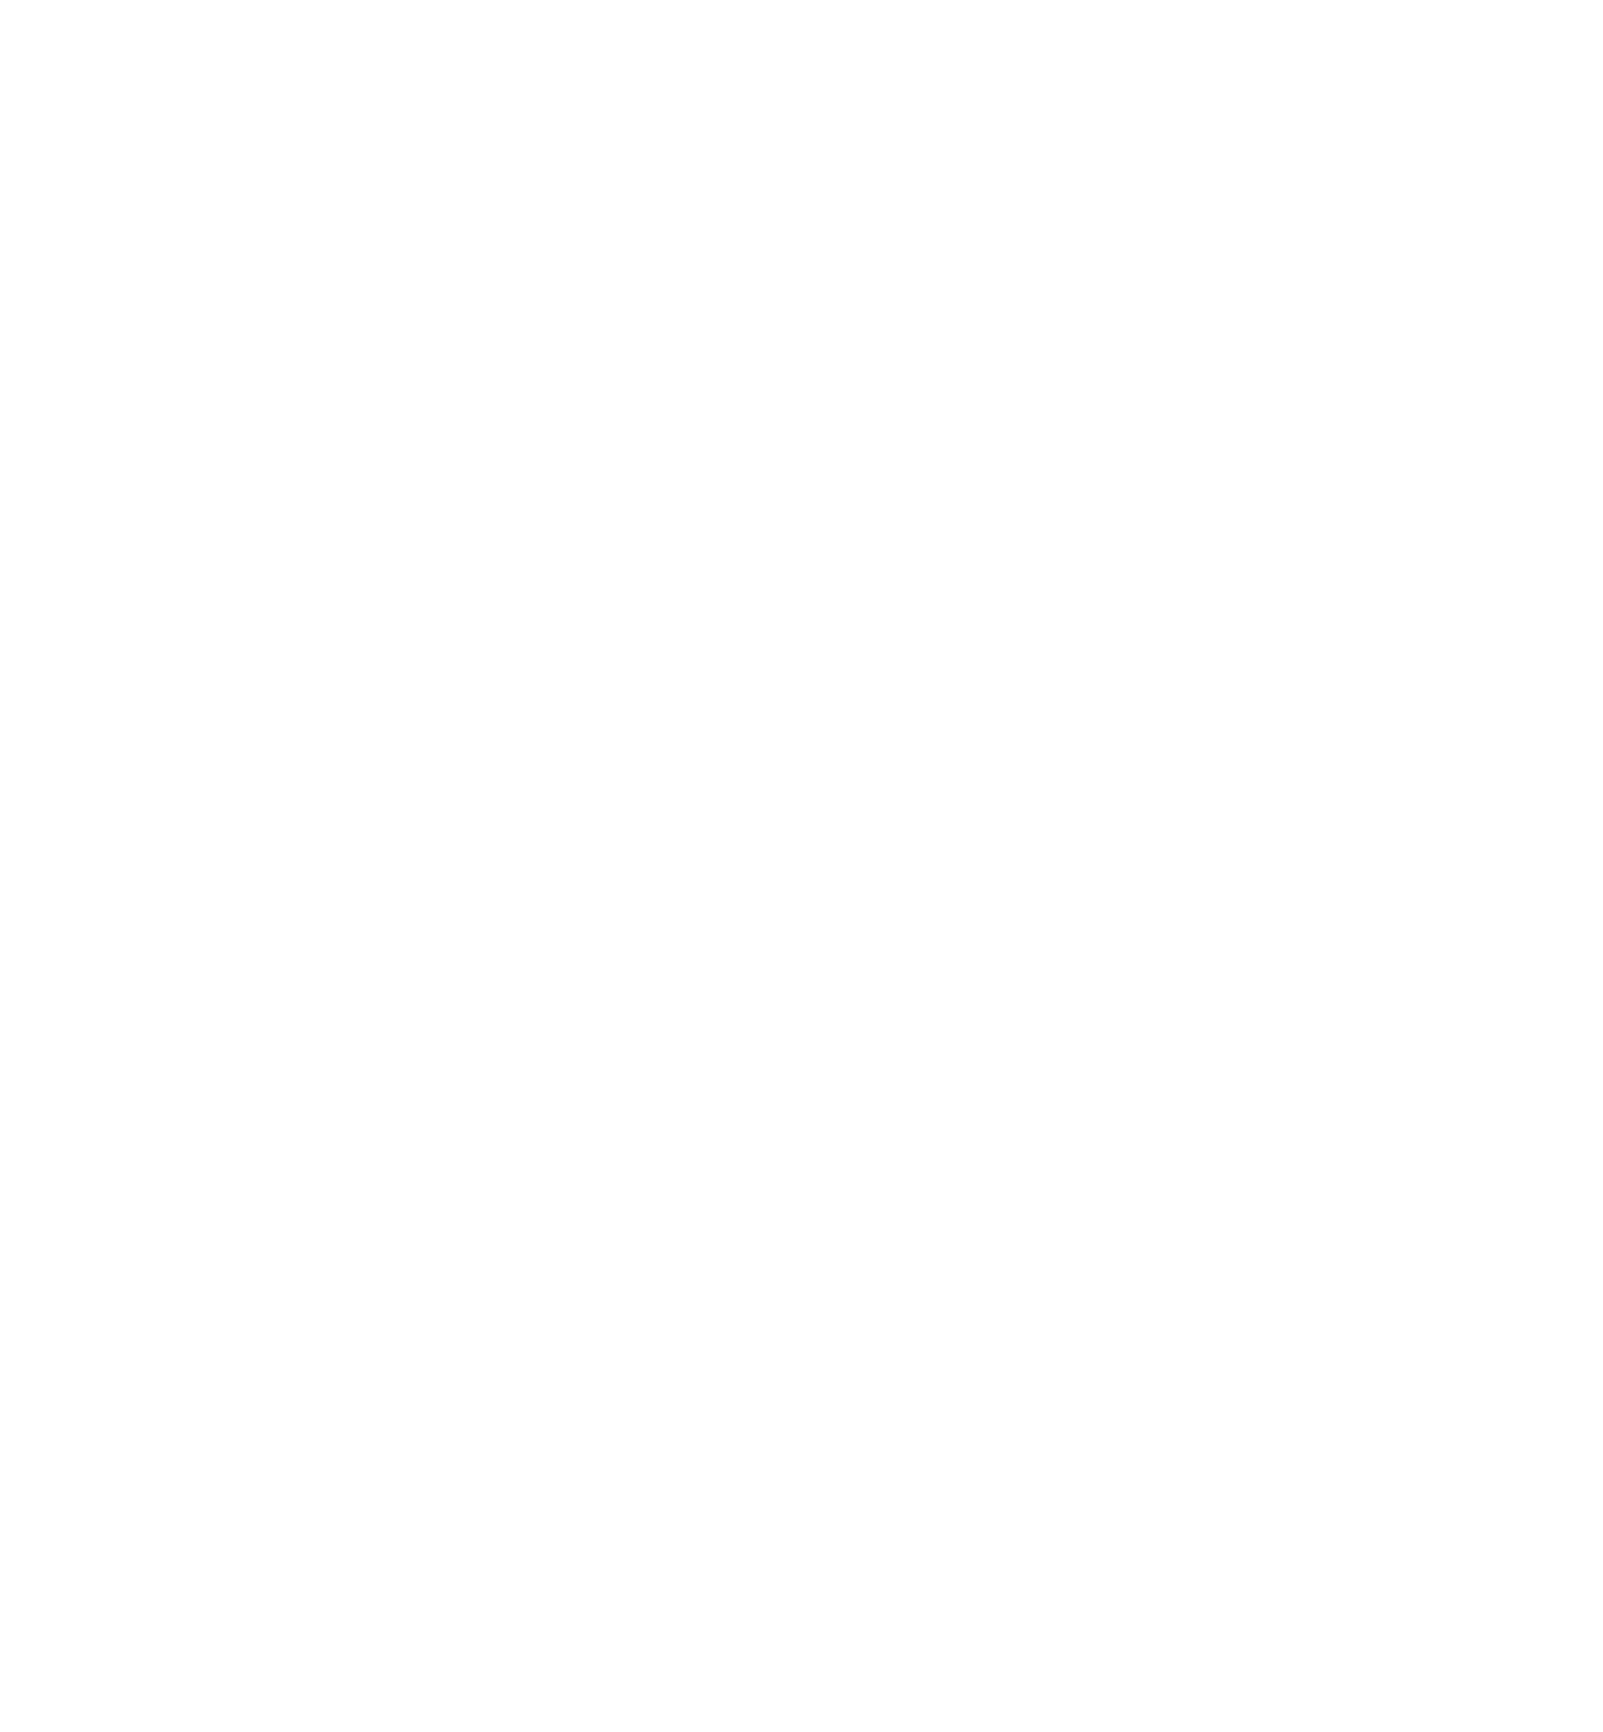
\includegraphics[width=\textwidth]{basketball-court.png}
        \column{.4\textwidth}
          \begin{itemize}
            \item \textbf{1 point} for free throws made after a foul by the other team
            \item \textbf{2 points} for shots made inside the 3-point line
            \item \textbf{3 points} for shots made outside the 3-point line
          \end{itemize}
      \end{columns}
    \end{frame}

    \begin{frame}[fragile]
\begin{knitrout}
\definecolor{shadecolor}{rgb}{0.137, 0.137, 0.137}\color{fgcolor}\begin{kframe}
\begin{alltt}
\hlkwd{plot}\hlstd{(nba}\hlopt{$}\hlstd{N3PA, nba}\hlopt{$}\hlstd{PTS,} \hlkwc{pch}\hlstd{=}\hlnum{16}\hlstd{,} \hlkwc{col}\hlstd{=}\hlstr{'orange'}\hlstd{,}
  \hlkwc{xlab}\hlstd{=}\hlstr{'Num 3-point shots attempted'}\hlstd{,} \hlkwc{ylab}\hlstd{=}\hlstr{'Total points'}\hlstd{)}
\end{alltt}
\end{kframe}
\includegraphics[width=\maxwidth]{/tmp/figures/unnamed-chunk-16-1} 

\end{knitrout}

    \end{frame}

    \begin{frame}[fragile]
      \fontsize{8}{8}\selectfont
\begin{knitrout}
\definecolor{shadecolor}{rgb}{0.137, 0.137, 0.137}\color{fgcolor}\begin{kframe}
\begin{alltt}
\hlstd{model1} \hlkwb{<-} \hlkwd{lm}\hlstd{(PTS} \hlopt{~} \hlstd{N3PA,} \hlkwc{data}\hlstd{=nba)}
\hlkwd{summary}\hlstd{(model1)}
\end{alltt}
\begin{verbatim}

Call:
lm(formula = PTS ~ N3PA, data = nba)

Residuals:
    Min      1Q  Median      3Q     Max 
-11.245  -2.511   0.055   2.225   8.640 

Coefficients:
            Estimate Std. Error t value Pr(>|t|)    
(Intercept)  86.1920     1.7746   48.57  < 2e-16 ***
N3PA          0.6484     0.0794    8.17  3.9e-13 ***
---
Signif. codes:  0 '***' 0.001 '**' 0.01 '*' 0.05 '.' 0.1 ' ' 1

Residual standard error: 3.5 on 118 degrees of freedom
Multiple R-squared:  0.361,	Adjusted R-squared:  0.356 
F-statistic: 66.8 on 1 and 118 DF,  p-value: 3.89e-13
\end{verbatim}
\end{kframe}
\end{knitrout}

    \end{frame}

    \begin{frame}{Can we do better?}
      \begin{center}
        $R^2=36\%$, so we can explain
        36\% of the variance in total points based only on
        knowing the number of 3-point attempts.

        \pause\bigskip

        This means that \textbf{most} of the variance (64\%) in total points is \textbf{not} explained by the number of 3-point attempts.

        \pause\bigskip

        Let's add another variable to our model --- why might 3-point percentage be useful as another predictor?
      \end{center}

    \end{frame}

    \begin{frame}[fragile]{Can we do better?}
      \fontsize{8}{8}\selectfont
\begin{knitrout}
\definecolor{shadecolor}{rgb}{0.137, 0.137, 0.137}\color{fgcolor}\begin{kframe}
\begin{alltt}
\hlstd{model2} \hlkwb{<-} \hlkwd{lm}\hlstd{(PTS} \hlopt{~} \hlstd{N3PA} \hlopt{+} \hlstd{PCT3P,} \hlkwc{data}\hlstd{=nba)}
\hlkwd{summary}\hlstd{(model2)}
\end{alltt}
\begin{verbatim}

Call:
lm(formula = PTS ~ N3PA + PCT3P, data = nba)

Residuals:
   Min     1Q Median     3Q    Max 
-8.349 -2.139 -0.079  1.869  9.190 

Coefficients:
            Estimate Std. Error t value Pr(>|t|)    
(Intercept)  62.0049     5.6140   11.04  < 2e-16 ***
N3PA          0.5647     0.0759    7.44  1.8e-11 ***
PCT3P         0.7342     0.1629    4.51  1.6e-05 ***
---
Signif. codes:  0 '***' 0.001 '**' 0.01 '*' 0.05 '.' 0.1 ' ' 1

Residual standard error: 3.2 on 117 degrees of freedom
Multiple R-squared:  0.456,	Adjusted R-squared:  0.447 
F-statistic:   49 on 2 and 117 DF,  p-value: 3.48e-16
\end{verbatim}
\end{kframe}
\end{knitrout}

    \end{frame}

    \begin{frame}{Can we do even better?}
      \begin{center}
        It would make sense that the \textbf{impact} of the number of 3-pointers taken on total points would \textbf{depend on} how well the team shoots the 3!

        \pause\bigskip

        This sounds like an interaction --- let's make a model with an interaction between the two predictors!
      \end{center}
    \end{frame}

    \begin{frame}[fragile]
      \fontsize{8}{8}\selectfont
\begin{knitrout}
\definecolor{shadecolor}{rgb}{0.137, 0.137, 0.137}\color{fgcolor}\begin{kframe}
\begin{alltt}
\hlstd{model3} \hlkwb{<-} \hlkwd{lm}\hlstd{(PTS} \hlopt{~} \hlstd{N3PA} \hlopt{*} \hlstd{PCT3P,} \hlkwc{data}\hlstd{=nba)}
\hlkwd{summary}\hlstd{(model3)}
\end{alltt}
\begin{verbatim}

Call:
lm(formula = PTS ~ N3PA * PCT3P, data = nba)

Residuals:
   Min     1Q Median     3Q    Max 
-7.263 -2.276  0.115  1.970  9.376 

Coefficients:
            Estimate Std. Error t value Pr(>|t|)    
(Intercept) 122.8490    30.5894    4.02  0.00011 ***
N3PA         -2.1190     1.3290   -1.59  0.11356    
PCT3P        -0.9841     0.8646   -1.14  0.25740    
N3PA:PCT3P    0.0756     0.0374    2.02  0.04542 *  
---
Signif. codes:  0 '***' 0.001 '**' 0.01 '*' 0.05 '.' 0.1 ' ' 1

Residual standard error: 3.2 on 116 degrees of freedom
Multiple R-squared:  0.474,	Adjusted R-squared:  0.461 
F-statistic: 34.9 on 3 and 116 DF,  p-value: 3.8e-16
\end{verbatim}
\end{kframe}
\end{knitrout}
    \end{frame}

    \begin{frame}[fragile]

      Model 3 corresponds to the regression equation
      \[
        \widehat{\text{PTS}} = 122.85
          - 2.12 \cdot\text{N3PA}
          - 0.98 \cdot\text{PCT3P}
          + 0.08 \cdot\text{N3PA}\cdot\text{PCT3P}.
      \]

      \pause

      We interpret the coefficients as follows:
      \begin{itemize}[<+->]
        \item \textbf{Intercept} (122.85) is our prediction of total points when $\text{N3PA}=\text{PCT3P}=0$. (Meaningless in this context!)
        \item \textbf{N3PA} ($-2.12$) is the predicted increase in total points for each additional 3-pointer taken, when $\text{PCT3P}=0$.
        \item \textbf{PCT3P} ($-0.98$)  is the predicted increase in total points for each additional percentage point of 3-point shooting accuracy, when $\text{N3PA}=0$.
        \item \textbf{$\text{N3PA}\cdot\text{PCT3P}$} ($0.08$) can be interpreted in two ways:\pause
          \begin{itemize}[<+->]
            \item the increase in the \emph{slope coefficient} for N3PA for each 1-unit increase of PCT3P.
            \item the increase in the \emph{slope coefficient} for PCT3P for each 1-unit increase of N3PA.
          \end{itemize}
      \end{itemize}
    \end{frame}

    \begin{frame}
\begin{knitrout}
\definecolor{shadecolor}{rgb}{0.137, 0.137, 0.137}\color{fgcolor}
\includegraphics[width=\maxwidth]{/tmp/figures/unnamed-chunk-21-1} 

\end{knitrout}
    \end{frame}

    \begin{frame}
\begin{knitrout}
\definecolor{shadecolor}{rgb}{0.137, 0.137, 0.137}\color{fgcolor}
\includegraphics[width=\maxwidth]{/tmp/figures/unnamed-chunk-22-1} 

\end{knitrout}
    \end{frame}

    \begin{frame}
\begin{knitrout}
\definecolor{shadecolor}{rgb}{0.137, 0.137, 0.137}\color{fgcolor}
\includegraphics[width=\maxwidth]{/tmp/figures/unnamed-chunk-23-1} 

\end{knitrout}

    \end{frame}
    \begin{frame}
      \[
        \widehat{\text{PTS}} = 122.85
          - 2.12 \cdot\text{N3PA}
          - 0.98 \cdot\text{PCT3P}
          + 0.08 \cdot\text{N3PA}\cdot\text{PCT3P}.
      \]

      \begin{itemize}
        \item How many points per game do you predict for a team that shoots 3-pointers at the NBA average rate (35.4) and that takes 30 3-pointers per game?
        \pause
        \item How bad would a team have to shoot the 3 before taking 3-point shots start to have a negative impact on total points?
      \end{itemize}
    \end{frame}

    \begin{frame}
\begin{knitrout}
\definecolor{shadecolor}{rgb}{0.137, 0.137, 0.137}\color{fgcolor}
\includegraphics[width=\maxwidth]{/tmp/figures/unnamed-chunk-24-1} 

\end{knitrout}
    \end{frame}
  \end{darkframes}
\end{document}
